\documentclass[11pt]{article}
\usepackage{amsmath, amssymb}
\usepackage{geometry}
\geometry{margin=1in}
\usepackage{fancyhdr}
\usepackage{lastpage}
\usepackage{parskip} % Better paragraph spacing
\usepackage{titlesec} % Better section formatting
\usepackage{graphicx}
\usepackage{float}
\usepackage[most]{tcolorbox}
\usepackage{lmodern}
\usepackage{caption}
\usepackage{hyperref}
\usepackage{listings}
\usepackage{xcolor}

\definecolor{codegreen}{rgb}{0,0.6,0}
\definecolor{codegray}{rgb}{0.5,0.5,0.5}
\definecolor{codepurple}{rgb}{0.58,0,0.82}
\definecolor{backcolour}{rgb}{0.95,0.95,0.92}

% Define code styling
\lstdefinestyle{mystyle}{
    backgroundcolor=\color{backcolour},
    commentstyle=\color{codegreen},
    keywordstyle=\color{magenta},
    numberstyle=\tiny\color{codegray},
    stringstyle=\color{codepurple},
    basicstyle=\ttfamily\footnotesize,
    breakatwhitespace=false,
    breaklines=true,
    captionpos=b,
    keepspaces=true,
    numbers=left,
    numbersep=5pt,
    showspaces=false,
    showstringspaces=false,
    showtabs=false,
    tabsize=2
}

\lstset{style=mystyle}

% Define commands for reusable content
\newcommand{\coursename}{CS-401 Applied Data Analysis}
\newcommand{\lecturenum}{10}
\newcommand{\lecturedate}{19/11/2025}
\newcommand{\professor}{Maria Brbic}

\hypersetup{colorlinks=true,linkcolor=blue,urlcolor=blue}

% Configure section spacing
\titlespacing*{\section}{0pt}{2ex plus 1ex minus .2ex}{1.5ex plus .2ex}
\titlespacing*{\subsection}{0pt}{1.5ex plus 1ex minus .2ex}{1ex plus .2ex}
% Header / Footer
\pagestyle{fancy}
\fancyhf{}
\fancyhead[L]{\coursename}
\fancyhead[R]{Lecture \lecturenum}
\fancyfoot[L]{EPFL - Computer Science}
\fancyfoot[C]{Author: Jonathan Dutoit}
\fancyfoot[R]{Page \thepage\ of \pageref{LastPage}}

\begin{document}

\begin{center}
  {\large EPFL - Computer Science} \\[0.5em]
  {\Large \textbf{\coursename}} \\[0.5em]
  {\large Lecture \lecturenum\ --- \lecturedate} \\[0.5em]
  {\large Author: Jonathan Dutoit} \\[0.5em]
  {\large Professor: \professor} \\[0.5em]
\end{center}

\vspace{2cm}

\begin{center}
  {\LARGE \textbf{Handling text data (Part 1)}}
\end{center}

\vspace{1cm}

\section*{Textual Data}

\begin{itemize}
	\item Much modern data is unstructured text
		\begin{itemize}
			\item Web
			\item Social media
			\item News
			\item Several ADA project datasets...
		\end{itemize}
	\item Frequently, "clean" datasets can be derived from "dirty" textual data:
		\begin{itemize}
			\item e.g., search queries are short texts; Google Trends time series for concepts are obtained by aggregating all search queries referring to the concept. 
		\end{itemize}
\end{itemize}

\textbf{Nov 2022: The Dawn of a New Era}: because of LLMs (ChatGPT). 

\section*{Outline}

\begin{itemize}
	\item 4 typical tasks on text data:
		\begin{itemize}
			\item Document retrieval
			\item Document classification
			\item Sentiment analysis
			\item Topic detection
		\end{itemize}
	\item How to phrase these tasks as machine learning problems
	\item How to pre-process text so it can be fed to ML algorithms
	\item ADA spirit: show you what's there; give you basic feel
\end{itemize}

\newpage
\vspace{0.5cm}

\begin{center}
	{\LARGE \textbf{Document Retrieval}} \\
	Typical task 1
\end{center}
\vspace{0.5cm}

\begin{itemize}
	\item \textbf{\textcolor{orange}{Given}}
		\begin{itemize}
			\item Document collections (a.k.a corpus)
			\item Query document (can be short query string)
		\end{itemize}
	\item \textbf{\textcolor{blue}{Task}}
		\begin{itemize}
			\item Rank all docs in collection by similarly to query
		\end{itemize}
	\item An old problem (e.g., libraries)
	\item Document retrieval is the core task solved by Web search engines ("10 blue links")
\end{itemize}

\section*{Document retrieval}

\begin{itemize}
	\item Straightforward approach: neighbor search (as in kNN)
	\item Define a distance function between documents
	\item Given query \textit{q}, find the \textit{k} docks with smallest distance to \textit{q}
	\item \textit{k} = 10, docs sorted by distance, blue links, ads $\Rightarrow$ Google
	\item The hard part: craft/learn a distance function (and scale it to the Web...)
\end{itemize}

\vspace{0.5cm}

\begin{center}
  {\LARGE \textbf{Document classification}} \\
  Typical task 2
\end{center}
\vspace{0.5cm}
\begin{itemize}
	\item \textbf{\textcolor{orange}{Given:}}
		\begin{itemize}
			\item Document \textit{d}
			\item Set of classes (e.g., topics: news, sports, tech, music, romance)
		\end{itemize}
	\item \textbf{\textcolor{blue}{Task:}}
		\begin{itemize}
			\item Decide to which one of the classes document \textit{d} belongs
		\end{itemize}
	\item Example scenario:
		\begin{itemize}
			\item Find gangster movies in CMU Movie Summary Corpus
		\end{itemize}
\end{itemize}

\section*{Document classifications}

\begin{itemize}
	\item Supervised learning 
	\item Obtain a large collection of documents
	\item Label each doc with the class it belongs to
	\item Represent docs as feature vectors
	\item Train a supervised classifier based on the labeled docs:
		\begin{itemize}
			\item e.g., kNN, logistic regression, decision tree, random forest, boosted decision trees, neural network, ...
		\end{itemize}
\end{itemize}

\vspace{0.5cm}

\begin{center}
  {\LARGE \textbf{Sentiment Analysis}} \\
  Typical task 3
\end{center}
\vspace{0.5cm}

\begin{itemize}
	\item \textcolor{orange}{\textbf{Given:}}
		\begin{itemize}
			\item Document \textit{d} (e.g., product review)
		\end{itemize}
	\item \textbf{\textcolor{blue}{Task:}}
		\begin{itemize}
			\item "Sentiment" score capturing how positive/negative \textit{d} is
		\end{itemize}
	\item Example scenarios:
		\begin{itemize}
			\item Infer what people think about a product from text only (i.e., without explicitly given ratings)
			\item Historical opinion analysis; e.g., how has people's attitude toward certain politicians changed over time?
		\end{itemize}
\end{itemize}
\section*{Sentiment analysis}
\begin{itemize}
	\item Supervised learning
		\begin{itemize}
			\item Regression
			\item Classification
		\end{itemize}	
	\item Same setup as for document classification:
		\begin{itemize}
			\item Label a training set with ground-truth sentiment scores
			\item Represent documents as features vectors
			\item Train supervised model: kNN, linear/logistic regression
		\end{itemize}
\end{itemize}

\vspace{0.5cm}

\begin{center}
  {\LARGE \textbf{Topic detection}} \\
  Typical task 4
\end{center}
\vspace{0.5cm}
\begin{itemize}
	\item \textcolor{orange}{\textbf{Given:}}
		\begin{itemize}
			\item Unlabeled document collections
		\end{itemize}
	\item \textbf{\textcolor{blue}{Task:}}
		\begin{itemize}
			\item Determine a set of prevalent topics in the docs
			\item Determine for each document to which topics it belongs
		\end{itemize}
	\item Example scenarios
		\begin{itemize}
			\item Detection of trending topics in social media (e.g., Twitter)
			\item Detection of distinct viewpoints on a political subject
			\item Exploratory analysis of a large doc collection
		\end{itemize}	
\end{itemize}

\section*{Topic detections}
\begin{itemize}
	\item Clustering
	\item Represent documents as feature vectors
	\item Run hierarchical or point-assignment clustering algorithm
		\begin{itemize}
			\item Hierarchical: agglomerative or divise
			\item Point-assignment: e.g., k-means, DBSCAN
		\end{itemize}
	\item Alternative: matrix factorization (next lecture)
\end{itemize}


\vspace{0.5cm}

\begin{center}
  {\LARGE \textbf{Feature Vectors}}
\end{center}
\vspace{0.5cm}

\textbf{Text is not immediately a feature vector}: variable length (even for fixed length); positions don't correspond to meaningful features. Text often doesn't have the format for directly running ML algorithms...

\begin{itemize}
	\item Need to transform arbitrarily long string to fixed-length vector
	\begin{itemize}
		\item Traditional and vetted: bag of words
		\item More recent: \textit{learn} a mapping from strings to vectors (buzzword: "text embedding")
	\end{itemize}
\end{itemize}

\section*{Bag of words}
\begin{itemize}
	\item Bag == multiset
		\begin{itemize}
			\item E.g., document "what you see is what you get" 
				\begin{itemize}
					\item bag of words \{get:1, is:1, see:1, what:2, you:2\}
				\end{itemize}
		\end{itemize}
	\item To have fixed-length representation for all documents:
		\begin{itemize}
			\item Vector with one entry for each unique word in vocabulary
			\item Bag-of-word vectors are very high-dimensional (typically 1e5 or 1e6) and very sparse
		\end{itemize}
\end{itemize}

\newpage
\textbf{An extra reason for sparsity: Zipf's law}

\begin{minipage}{0.6\textwidth}
\textbf{The probability of observing a word scales inversely with its frequency rank:} \\
\[
p(w_i) \propto 1/i
.\] \\
(where $w_i$ is the \textit{i}-th most frequent word)
\end{minipage}
\hfill
\begin{minipage}{0.4\textwidth}
\centering
Word frequency and rank in \textit{Romeo and Juliet} (linear-linear)
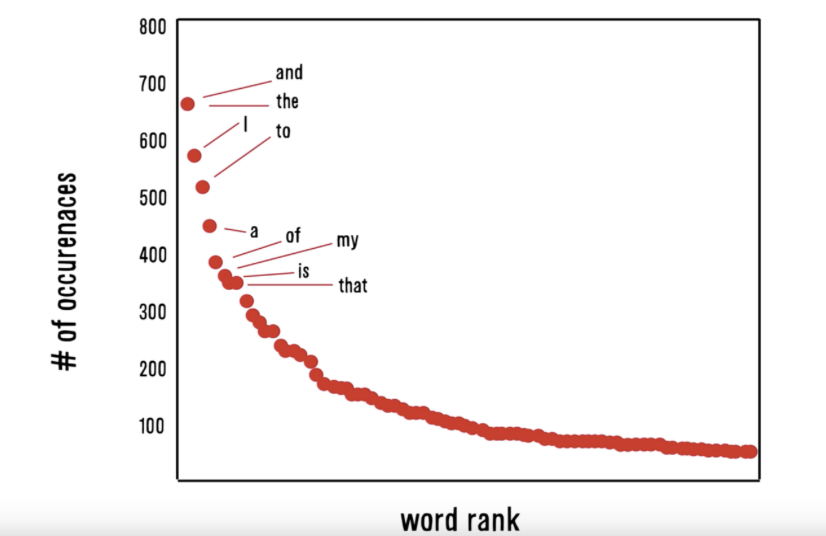
\includegraphics[width=\linewidth]{zipfs}
\textit{we care more about the tail here because they contain more important information}
\end{minipage}

\section*{Bag-of-words matrix}
\begin{itemize}
	\item Combine document vectors as rows in a matrix
		\begin{itemize}
			\item One row per doc
			\item One column per word in vocabulary
		\end{itemize}
	\item This matrix is huge!
		\begin{itemize}
			\item E.g., Wikipedia: 6M docs, 2M words $\Rightarrow$ 12 trillion entries
		\end{itemize}
	\item Solution: use a sparse matrix format
		\begin{itemize}
			\item Triples: (\verb|doc_idx|, \verb|word_idx|, \verb|count|)
			\item E.g., Wikipedia, assuming 2000 words per article on avg.: 12 billion non-zero entries (fits in memory)
		\end{itemize}
	\item With matrix representation, you're almost ready to use any ML model
		\begin{itemize}
			\item Be careful when mapping raw text to bag-of-words matrix!
				\begin{itemize}
					\item Character encoding
					\item Language identification
					\item Tokenisation
					\item Stopword removal
					\item Word normalization
				\end{itemize}
			\item Tweaking the matrix a bit can lead to much better performance
				\begin{itemize}
					\item Re-weight/normalize rows and/or columns of matrix
				\end{itemize}
		\end{itemize}
\end{itemize}

\vspace{0.5cm}
\newpage
\begin{center}
  {\LARGE \textbf{Bag of tricks for bags of words}}
\end{center}
\vspace{0.5cm}

\section*{Character encoding}
\begin{itemize}
	\item Mapping from (abstract) characters to bytes
	\item Old school: ASCII, Latin-1; new school: Unicode (e.g., UTF-8, UTF-16, UTF-32)
	\item E.g., W $\Rightarrow$ 0x57 (one byte)
	\item Reading text from file:
		\begin{itemize}
			\item Need to read with encoding that was used to write file
			\item Especially important for non-English text: à, ê, ü, ...
		\end{itemize}
	\item Writing to file: Always use UTF-8 or UTF-16; hard-code the output format!
	\item Otherwise, your future self will be very angry at you
\end{itemize}

\section*{Language identification}
\begin{itemize}
	\item Typically, you're interested in text from a single language
	\item Increasingly, content is multilingual (e.g., Twitter, Wikipedia)
	\item Ideally, language code is specified (e.g., headers in HTML; JSON field in Twitter API results)
	\item But not always... For this, there are good libraries
		\begin{itemize}
			\item Most commonly based on letter trigrams (e.g., "eau", "ghi", "ijs", "sch", "eiss", "ção", "prv")
			\item Much harder if you messed up character encoding...
		\end{itemize}
\end{itemize}

\section*{Tokenization}
\begin{itemize}
	\item Maps character string into sequence of tokens ($\approx$ words)
	\item E.g., "Hello! How are you?" $\Rightarrow$ \verb|Hello_!_How_are_you_?|
	\item Tempting to do this yourself by splitting at white spaces and punctuation. But there are many corner cases like emoticons, question and exclamation marks together, ...
	\item Don't do it yourself, use libraries instead; e.g., 
		\begin{itemize}
			\item Python: spaCy, nltk; Java; Standford CoreNLP
			\item Rule-based, deterministic, fast
		\end{itemize}
	\item Optimal tokenizer different for different languages, but English tokeniser is often good enough for Latin languages. But in Chinese's there's no white space between words or for \textbf{compound works} like in German.
\end{itemize}

\section*{Stopword removal}
\begin{itemize}
	\item Very frequent, "small" words carry little information for most tasks and can "drown out" information contained in real content words
	\item E.g., "a", "the", "is", "you", "I", punctuation marks
	\item Many stopword lists online, but be careful!
		\begin{itemize}
			\item Different tasks require removing different stopwords
			\item Good heuristic: remove words appearing in at least \textit{p\%} of all documents (but what should \textit{p} be...?)
			\item Sometimes stopword removal hurts!
			\begin{itemize}
				\item Author identification, psychological modeling; punctuation can be useful as well: e.g., "!!!", ":-)"
			\end{itemize}
		\end{itemize}
\end{itemize}

\section*{Word normalization: casefolding}

\begin{itemize}
	\item E.g., "I love yams. Yams are yummy."
	\item Should "yams" and "Yams"really be different features?
	\item Simple solution: make everything lower-vase ("casefolding")
	\item But then "I'd rather have an apple than an Apple.": the phrase loses its sense with casefolding
	\item Hand-code exceptions? In practice (especially when dataset is large), typically best to \textbf{not} do casedfolding
	\item But when dataset is small, might help because less sparsity. 
\end{itemize}

\section*{Word normalization: Stemming}
\begin{itemize}
	\item Map different forms of same word to same, normalized form, by stripping affixes
	\item E.g., "walking", "walks", "walked" $\Rightarrow$ "walk"
	\item Typically done in hacky, heuristic way
	\item Pros: decreases sparsity in bag-of-words matrix
	\item Con: discard information
		\begin{itemize}
			\item E.g., "business" vs. "busy"; "operating" (as in "operating system")
		\end{itemize}
	\item In English (esp. with big data) typically not done anymore. Still very useful in morphologically richer languages (e.g., Bantu languages)
\end{itemize}

\section*{Word normalization: Lemmatization}
\begin{itemize}
	\item Lemmatization == stemming++
	\item Map tokens to lexicon entries
	\item E.g., "U.S.A.", "US" $\Rightarrow$ "United States" \\
		"You \textbf{lie} in the grass" vs. "You \textbf{lie} to me"
	\item Frequently omitted, as it requires complete lexicon and complex mapping rules
	\item Especially hard for non-English
\end{itemize}

\vspace{0.5cm}
\section*{Social Media}

A real tweet: "ikr smh he asked fir yo last name so he can add u on fb lololol"

Need dedicated toolkits such as \textbf{TweenNLP} because of necessary abbreviation, common repeating letters/syllables, ...

\section*{Tokens vs. n-grams}
\begin{itemize}
	\item So far: bag-of-words matrix
		\begin{itemize}
			\item Rows: documents
			\item Columns: tokens (a.k.a. unigrams, or 1-grams)
		\end{itemize}
	\item Frequently, longer sequences belong together
		\begin{itemize}
			\item E.g., "United States", "operating system"
		\end{itemize}
	\item Brute-force approach: use $n > 1$
		\begin{itemize}
			\item E.g., all bigrams (n = 2), all trigrams (n = 3)
			\item Using all 5-grams can beat neural networks
			\item Problem: combinatorial explosion
		\end{itemize}
\end{itemize}
\textbf{Smarter}:
\begin{itemize}
	\item Feature selection ("multi-word expressions", "phrase extraction")
	\item Simple approach for bigrams: keep bigram if \textit{mutual information} between constituent tokens is large
	\item How to generalize to $n > 2$? 
		\begin{itemize}
			\item Frequent itemset/sequence mining
			\item Wikipedia anchor texts
			\item Compressive feature learning
		\end{itemize}
\end{itemize}

\vspace{0.5cm}

\begin{center}
  {\LARGE \textbf{Postprocessing the BOW matrix}}
\end{center}
\vspace{0.5cm}
\section*{Inverse document frequency}

\begin{itemize}
	\item Not all words equally informative. This is the reason for removing stopwords ("a", "the", "is", ...)
	\item Beyond discarding stopwords, want to give less weight to more common words
		\begin{itemize}
			\item E.g., "per" vs. "perceptron"
		\end{itemize}
	\item Standard way: \textbf{IDF = inverse document frequency}
		\begin{itemize}
			\item docfreq(\textit{w}): number of documents that contain word \textit{w}
			\item \textit{N}: overall number of documents
			\item idf(\textit{w}) = $-\log(docfreq(w) / N) = \log{N} - \log(docfreq(w))$
			\item Interpretation: information content (in term of #bits) of event "randomly drawing a document that contains \textit{w}"
			\item Beyond this theoretical justification, IDF weighting has been show to work well in practice. 
		\end{itemize}
\end{itemize}

\section*{TF-IDF matrix}
\begin{itemize}
	\item tf(\textit{d, w}): term frequency of word \textit{w} in doc \textit{d}
		\begin{itemize}
			\item This is what the bag of words captures
			\item E.g., document "what you see is what you get" $\Rightarrow$ \{get:1, is:1, see:1, what:2, you:2\}
		\end{itemize}
	\item idf(\textit{w}): inverse doc freq of \textit{w} (computed on entire corpus)
	\item TF-IDF matrix: 
		\begin{itemize}
			\item Entry in row \textit{d} and column \textit{w} has value tf(\textit{d, w}) $\cdot$ idf(\textit{w})
			\item Amounts to multiplying column \textit{w} with constant idf(\textit{w})
		\end{itemize}
\end{itemize}

\section*{Row normalization of TF-IDF matrix}
\begin{itemize}
	\item Longer docs have more non-zero entries
	\item Interpreted as vectors, longer docs have longer vectors
	\item This may throw off ML algorithms
		\begin{itemize}
			\item Long vectors far away from short vectors
			\item Dot product: random vector has higher dot product with longer vector
		\end{itemize}
	\item Fix: normalize doc vectors, i.e., rows of TF-IDF matrix
		\begin{itemize}
			\item L2-normalization: all rows have Euclidean distance 1 from origin (all data points lie on a unit sphere)
			\item L1-normalization: all rows sum to 1, i.e., can be interpreted as distribution
		\end{itemize}
	\item How to know which one is better? \textbf{Cross-validation}!
\end{itemize}

\section*{Column normalization}
\begin{itemize}
	\item IDF-scaling may be seen as column normalization
	\item Additionally, it may help to apply any of the normalization techniques we discussed in lecture 8 ("Applied ML")
		\begin{itemize}
			\item Min-max scale
			\item Standardize: subtract mean; divide by standard deviation
		\end{itemize}
	\item How to know which one (if any) to use? \textbf{Cross-validation}!
\end{itemize}


\end{document}
